\documentclass[]{article}
\usepackage{lmodern}
\usepackage{amssymb,amsmath}
\usepackage{ifxetex,ifluatex}
\usepackage{fixltx2e} % provides \textsubscript
\ifnum 0\ifxetex 1\fi\ifluatex 1\fi=0 % if pdftex
  \usepackage[T1]{fontenc}
  \usepackage[utf8]{inputenc}
\else % if luatex or xelatex
  \ifxetex
    \usepackage{mathspec}
  \else
    \usepackage{fontspec}
  \fi
  \defaultfontfeatures{Ligatures=TeX,Scale=MatchLowercase}
\fi
% use upquote if available, for straight quotes in verbatim environments
\IfFileExists{upquote.sty}{\usepackage{upquote}}{}
% use microtype if available
\IfFileExists{microtype.sty}{%
\usepackage{microtype}
\UseMicrotypeSet[protrusion]{basicmath} % disable protrusion for tt fonts
}{}
\usepackage[margin=2cm]{geometry}
\usepackage{hyperref}
\hypersetup{unicode=true,
            pdftitle={Early warning signals derived from COVID-19 testing data},
            pdfauthor={Christopher M. Hoover, Joshua Schwab, Maya Peterson, Mark van der Laan, others},
            pdfborder={0 0 0},
            breaklinks=true}
\urlstyle{same}  % don't use monospace font for urls
\usepackage{graphicx,grffile}
\makeatletter
\def\maxwidth{\ifdim\Gin@nat@width>\linewidth\linewidth\else\Gin@nat@width\fi}
\def\maxheight{\ifdim\Gin@nat@height>\textheight\textheight\else\Gin@nat@height\fi}
\makeatother
% Scale images if necessary, so that they will not overflow the page
% margins by default, and it is still possible to overwrite the defaults
% using explicit options in \includegraphics[width, height, ...]{}
\setkeys{Gin}{width=\maxwidth,height=\maxheight,keepaspectratio}
\IfFileExists{parskip.sty}{%
\usepackage{parskip}
}{% else
\setlength{\parindent}{0pt}
\setlength{\parskip}{6pt plus 2pt minus 1pt}
}
\setlength{\emergencystretch}{3em}  % prevent overfull lines
\providecommand{\tightlist}{%
  \setlength{\itemsep}{0pt}\setlength{\parskip}{0pt}}
\setcounter{secnumdepth}{0}
% Redefines (sub)paragraphs to behave more like sections
\ifx\paragraph\undefined\else
\let\oldparagraph\paragraph
\renewcommand{\paragraph}[1]{\oldparagraph{#1}\mbox{}}
\fi
\ifx\subparagraph\undefined\else
\let\oldsubparagraph\subparagraph
\renewcommand{\subparagraph}[1]{\oldsubparagraph{#1}\mbox{}}
\fi

%%% Use protect on footnotes to avoid problems with footnotes in titles
\let\rmarkdownfootnote\footnote%
\def\footnote{\protect\rmarkdownfootnote}

%%% Change title format to be more compact
\usepackage{titling}

% Create subtitle command for use in maketitle
\newcommand{\subtitle}[1]{
  \posttitle{
    \begin{center}\large#1\end{center}
    }
}

\setlength{\droptitle}{-2em}

  \title{Early warning signals derived from COVID-19 testing data}
    \pretitle{\vspace{\droptitle}\centering\huge}
  \posttitle{\par}
    \author{Christopher M. Hoover, Joshua Schwab, Maya Peterson, Mark van der Laan,
others}
    \preauthor{\centering\large\emph}
  \postauthor{\par}
    \date{}
    \predate{}\postdate{}
  
\usepackage{booktabs}
\usepackage{longtable}
\usepackage{array}
\usepackage{multirow}
\usepackage{wrapfig}
\usepackage{float}
\usepackage{colortbl}
\usepackage{pdflscape}
\usepackage{tabu}
\usepackage{threeparttable}
\usepackage{threeparttablex}
\usepackage[normalem]{ulem}
\usepackage{makecell}
\usepackage{xcolor}

\begin{document}
\maketitle

\hypertarget{abstract}{%
\subsection{Abstract}\label{abstract}}

COVID19 testing data is essential to monitor the status of ongoing
epidemics across the U.S. and the world. Because of the high rate of
asymptomatic and mildly symptomatic cases that contribute to
transmission, widespread testing and subsequent contact tracing and
isolation are necessary to reduce epidemic spread The effective
reproductive rate, \(\mathcal{R}_e\), is a simple measure of
transmission interpreted as the expected number of new infections
arising from a single infection at a given time, that can be used to
monitor the status of an outbreak. Here we discuss estimation of
\(\mathcal{R}_e\) from currently available testing data and proprose
methods to correct for inherent biases that currently limit the utility
of testing as a reliable indicator of the status of the COVID19
pandemic.

\hypertarget{background}{%
\section{Background}\label{background}}

\hypertarget{covid19}{%
\subsection{COVID19}\label{covid19}}

Areas across the United States and the world are beginning to reopen
following the unprecedented pandemic caused by the emergence of
SARS-CoV2. Widespread availability of testing for active and past
infections remains a critical component of the ongoing response to the
COVID19 pandemic\ldots{}

\hypertarget{testing}{%
\subsection{Testing}\label{testing}}

\begin{itemize}
\tightlist
\item
  Background on types of tests\\
\item
  What tests are actually doing (e.g.~distingiush PCR = active
  infections, antibody = past infections)

  \begin{itemize}
  \tightlist
  \item
    Sensitivity issues
  \end{itemize}
\end{itemize}

\hypertarget{testing-can-be-earliest-indicator-of-rising-infections-if-conductedanalyzed-appropriately}{%
\subsubsection{Testing can be earliest indicator of rising infections if
conducted/analyzed
appropriately}\label{testing-can-be-earliest-indicator-of-rising-infections-if-conductedanalyzed-appropriately}}

Hospitalizations and deaths are more what we're worried about, but these
are preceded in time by increase in cases. Since tests can detect
infection before these more severe outcomes, they can be an earlier
indicator of increases in transmission. A useful summary statistic to
estimate the current status of an outbreak is \(\mathcal{R}_e\), the
expected number of additional cases caused by a single case at any time
during the outbreak {[}CITE{]}.

\hypertarget{testing-cannot-currently-be-used-to-reliably-estimate-mathcalr_e-because-of-bias-due-to-variability-in-test-seeking-behaviors-test-availability-geographically-socioeconomically-etc.}{%
\subsubsection{\texorpdfstring{Testing cannot currently be used to
reliably estimate \(\mathcal{R}_e\) because of bias due to variability
in test-seeking behaviors, test availability (geographically,
socioeconomically,
etc.)}{Testing cannot currently be used to reliably estimate \textbackslash mathcal\{R\}\_e because of bias due to variability in test-seeking behaviors, test availability (geographically, socioeconomically, etc.)}}\label{testing-cannot-currently-be-used-to-reliably-estimate-mathcalr_e-because-of-bias-due-to-variability-in-test-seeking-behaviors-test-availability-geographically-socioeconomically-etc.}}

Testing can be used in either passive or active surveillance to monitor
the status of ongoing outbreaks. Especially early in the outbreak when
testing was not widely available, the set of individuals allowed (wc?)
to be tested was restricted. To date, most COVID19 testing data has been
passively collected: those with suspected COVID19 exposure or symptoms
seek out testing from a healthcare provider, rather than actively being
pursued to be tested in a more systematic fashion, e.g.~as part of a
representative cohort of the population of interest. This introduces
considerable bias into epidemiological estimates derived from the
testing data, such as \(\mathcal{R}_e\). {[}Review CITEs on passive
surveillance and bias{]} The number of tests available, test-seeking
behaviors of different populations/individuals, and {[}something else{]}
all influence the number of positive tests and the positive test percent
in a given location and time (Figure 1, W2; \textbf{Maybe could add
\(\mathcal{R}_e\) to the DAG as a function of \(Y\)?}).

Crude metrics from testing data such as the number of positive tests
reported or the percent of tests conducted that are positive have
been/are being used to monitor the status of outbreaks across the
US/world. However, such metrics are heavily biased due to reasons
outlines above, and may be flawed representations of true underlying
infection dynamics such as \(\mathcal{R}_e\) {[}\textbf{Think this
sentence/point is really important and could use some work}{]}. Here we
propose/review methods for correcting for these underlying biases in
testing data, discuss their pros and cons, and evaluate their ability to
a) estimate \(\mathcal{R}_e\) in real time and b) predict a future
increase in hospitalizations that will overwhelm capacity. We conclude
by proposing methods to generate unbiased testing data prospectively
using adaptive design (active surveillance, embedding prospective
cohorts within passive testing, all/none of the above?) and
{[}hopefully{]} show that these methods outperform those currently
available that rely on inherent flaws in currently available testing
data.

\begin{figure}
\centering
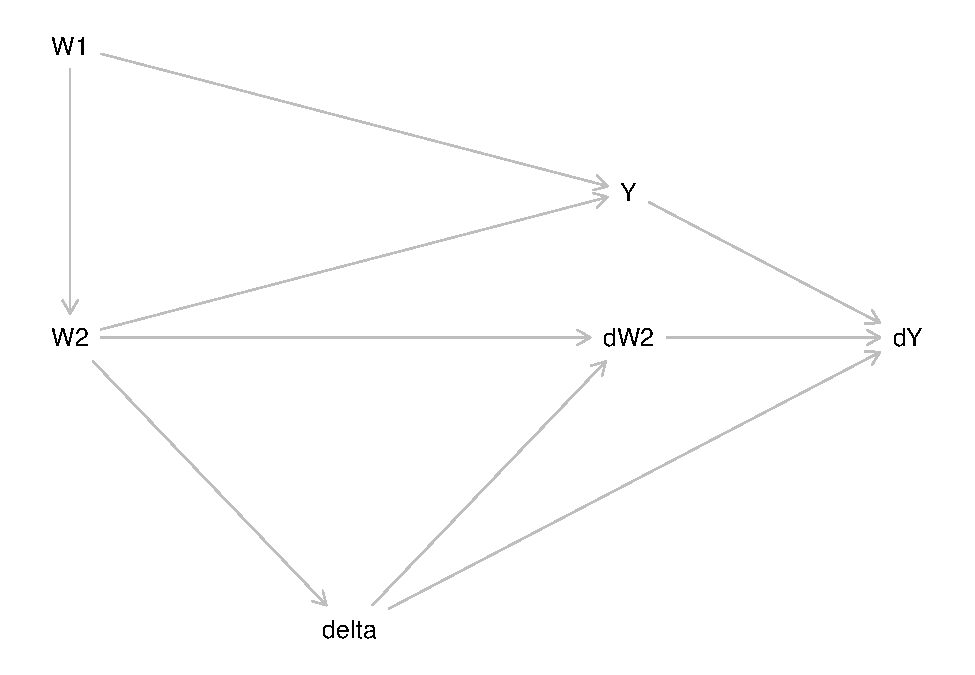
\includegraphics{Testing_Writeup_files/figure-latex/dag-1.pdf}
\caption{TODO: Make this longitudinal? Data generating process for
COVID19 testing data where W1 is demographic covariates (age, race,
SES), W2 is risk covariates (symptoms, contacts), Y is SARS-CoV2
infection status, delta is testing status. The observed data \(O\)
consists of (\(W_1, delta, dW2, dY\)), but conditioing on \(W_2\) is
necessary to identify \(E(Y)\).}
\end{figure}

\hypertarget{correcting-for-biasaccurate-estimation-of-eyadjusting-for-w2}{%
\section{\texorpdfstring{Correcting for bias/Accurate estimation of
\(E(Y)\)/Adjusting for
\(W2\)}{Correcting for bias/Accurate estimation of E(Y)/Adjusting for W2}}\label{correcting-for-biasaccurate-estimation-of-eyadjusting-for-w2}}

\begin{table}

\caption{\label{tab:tab1}Methods to estimate E(Y)}
\centering
\resizebox{\linewidth}{!}{
\begin{tabular}[t]{llll}
\toprule
Method & Pros & Cons & Reference\\
\midrule
Number of positive tests & real-time, simple, no analysis required & Heavily biased by number of tests conducted, test-seeking behaviors, etc & \\
Percent of tests conducted that are positive & Real-time, simple, removes bias from number of tests conducted & Heavily biased by test-seeking behaviors, etc. & \\
Adjustment from additional epidemiological data & Removes bias associated with test-seeking & Delay between infection and hospitalization/death means unable to estimate in real-time & LSHTM\\
Adjustment from additional demographic/survey? data & Simple and straightforward & Does not adequately control for confounding by W2, requires linelist testing data & \\
Fitting dynamic models & Real-time, draws on multiple data sources to control for biases & Identifiable?, complex and computationally intensive & \\
\bottomrule
\end{tabular}}
\end{table}

\hypertarget{approaches}{%
\subsection{Approaches}\label{approaches}}

\hypertarget{data-generating-process}{%
\subsubsection{Data-generating process}\label{data-generating-process}}

Needs to:

\begin{itemize}
\tightlist
\item
  Accurately represent influence of W1 and W2 on transmission\\
\item
  Accurately represent influence of W1 and W2 on testing (both simulated
  and observed)\\
\item
  Allow easy manipulation/implementation of changes in
  \(\mathcal{R}_e\)\\
\item
  Track infection and testing status across different (SES, race,
  demographic, occupational?) groups
\end{itemize}

\hypertarget{candidates}{%
\paragraph{Candidates:}\label{candidates}}

\begin{itemize}
\tightlist
\item
  Agent-based model\\
\item
  Branching-process model with network influence\\
\item
  Something simpler may be adequate for the point that testing isn't
  great and could be improved
\end{itemize}

\hypertarget{estimation-from-raw-testing-data}{%
\subsubsection{Estimation from raw testing
data}\label{estimation-from-raw-testing-data}}

Either number of positive tests or pct positive tests

\hypertarget{adjustment-from-additional-data-sources-demographic-age-race-zip-ses-andor-epidemiologic-hospitalizations-and-deaths}{%
\subsubsection{Adjustment from additional data sources (demographic
{[}Age, Race, Zip, SES{]} and/or epidemiologic {[}hospitalizations and
deaths{]})}\label{adjustment-from-additional-data-sources-demographic-age-race-zip-ses-andor-epidemiologic-hospitalizations-and-deaths}}

\hypertarget{lshtm-method-case-fatality-ratio-adjustment}{%
\paragraph{LSHTM method (Case-fatality ratio
adjustment?)}\label{lshtm-method-case-fatality-ratio-adjustment}}

\begin{itemize}
\tightlist
\item
  Time-delay limits utility\\
\item
  See
  \href{https://cmmid.github.io/topics/covid19/global_cfr_estimates.html}{this
  LSHTM report} for one method that seems to be widely accepted\\
\item
  I worked briefly on trying to derive a max likelihood estimate of
  COVID19 cases on day t from hospitalizations and deaths, but got stuck
  on right censoring. Could revive that effort though
\end{itemize}

\hypertarget{adjustment-built-into-model-fitting}{%
\subsubsection{Adjustment built into model
fitting}\label{adjustment-built-into-model-fitting}}

Big question: How inherently different is this really from methods
above? Just a combination of them?

\hypertarget{approach-chris-has-been-working-on}{%
\paragraph{Approach Chris has been working
on}\label{approach-chris-has-been-working-on}}

\begin{itemize}
\tightlist
\item
  Still relies on additional data sources for fitting\\
\item
  Projections require assumptions of number of tests, bias in testing in
  the future
\end{itemize}

\hypertarget{improving-testing-is-this-another-paper-even}{%
\section{Improving testing (Is this another paper
even??)}\label{improving-testing-is-this-another-paper-even}}

\begin{itemize}
\tightlist
\item
  What additional data can be reported to improve epi estimates (Symptom
  status, age, etc.)\\
\item
  Can additional data be collected in order to improve the utility of
  available testing resources

  \begin{itemize}
  \tightlist
  \item
    Intuition is that smart reallocation of testing to do some active
    surveillance will improve estimation even more than just doing more
    tests, which I think could/should be one of the main messages\\
  \item
    Could maybe start with data from the Mission Study, use it to derive
    age/race/income? adjusted rates for all of SF, compare to testing
    data reported for all of SF county at the same time. Could provide
    an initial estimate of testing bias. Would be even better if we
    could do record linkage between Mission Study and other testing data
  \end{itemize}
\end{itemize}


\end{document}
